\def\SECTION{3.4 Perpendicular Lines}
\documentclass[aspectratio=169,14pt]{beamer}
\usepackage[T1]{fontenc}
\usepackage{mathpazo}
\usepackage{amsmath,amssymb}
\usepackage{tikz}
\usetikzlibrary{arrows.meta,calc,decorations.pathreplacing}
\definecolor{fblue}{HTML}{1F4E79}
\definecolor{fteal}{HTML}{0F7C7C}
\definecolor{fgold}{HTML}{C9962B}
\definecolor{fred}{HTML}{B3261E}
\definecolor{fink}{HTML}{16233B}
\definecolor{fsoft}{HTML}{EEF3F8}
\definecolor{fgoldsoft}{HTML}{FBF1DC}
\setbeamertemplate{navigation symbols}{}
\setbeamercolor{normal text}{fg=fink}
\setbeamercolor{frametitle}{fg=fblue}
\setbeamerfont{frametitle}{series=\bfseries,size=\Large}
\setbeamercolor{structure}{fg=fteal}
\setbeamertemplate{itemize item}{\color{fteal}$\blacktriangleright$}
\setbeamertemplate{frametitle}{\vspace{6pt}\insertframetitle\par\vspace{-2pt}{\color{fgold}\rule{2.2cm}{2pt}}}
\setbeamertemplate{footline}{\hspace{0.6cm}{\color{fblue}\scriptsize\bfseries Fang\textcolor{fteal}{Math}}\hfill{\scriptsize\color{gray}\SECTION\quad\insertframenumber}\hspace{0.6cm}\vspace{6pt}}
\newcommand{\key}[1]{{\color{fteal}\textbf{#1}}}
\newcommand{\ans}[1]{\colorbox{fgoldsoft}{\color{fink}\ensuremath{#1}}}
\newcommand{\warn}[1]{\begin{beamercolorbox}[sep=8pt,rounded=true]{warnbox}{\color{fred}\textbf{Watch out!}}\enskip #1\end{beamercolorbox}}
\setbeamercolor{warnbox}{bg=fred!8,fg=fink}
\setbeamercolor{turnbox}{bg=fgoldsoft,fg=fink}
\setbeamercolor{defbox}{bg=fsoft,fg=fink}
\newcommand{\defn}[1]{\begin{beamercolorbox}[sep=8pt,rounded=true]{defbox}#1\end{beamercolorbox}}
\newenvironment{yourturn}{\begin{beamercolorbox}[sep=10pt,rounded=true]{turnbox}{\color{fgold}\Large\bfseries Your turn!}\quad{\small Pause the video and try it.}\par\medskip}{\end{beamercolorbox}}
\newcommand{\titleframe}[3]{%
\begin{frame}[plain]
\begin{tikzpicture}[remember picture,overlay]
\fill[fblue] (current page.north west) rectangle ([yshift=-0.9cm]current page.north east);
\node[anchor=west,text=white,font=\bfseries] at ([xshift=0.6cm,yshift=-0.45cm]current page.north west) {Fang\textcolor{fgold}{Math}};
\node[anchor=east,text=white,font=\small] at ([xshift=-0.6cm,yshift=-0.45cm]current page.north east) {Geometry $\cdot$ Chapter \CHNO};
\end{tikzpicture}
\vfill
{\color{fteal}\large\bfseries #1}\par\medskip
{\color{fblue}\fontsize{30}{34}\selectfont\bfseries #2}\par\medskip
{\color{fgold}\rule{3cm}{3pt}}\par\bigskip
{\large #3}
\vfill
{\small\color{gray} fangmath.com $\cdot$ YouTube @fangmathcom}
\end{frame}}
\newcommand{\closeframe}[1]{%
\begin{frame}{Remember}
#1
\vfill
\begin{center}{\color{fblue}\large\bfseries Now practice at your level:}\par\smallskip
{\Large\color{fteal}\bfseries fangmath.com} \enskip{\color{gray}$\to$ Geometry $\to$ Chapter \CHNO}\end{center}
\end{frame}}

\usepackage{pgfplots}\pgfplotsset{compat=1.17}
\newcommand{\grid}[4]{\draw[step=1,gray!25] (#1,#2) grid (#3,#4);\draw[-{Stealth},gray] (#1,0)--(#3+0.3,0) node[right]{\small$x$};\draw[-{Stealth},gray] (0,#2)--(0,#4+0.3) node[above]{\small$y$};}
\def\CHNO{3}
\usetikzlibrary{angles,quotes}
\begin{document}
\titleframe{Lesson 3.4}{Perpendicular Lines}{Right angles, and the shortest distance to a line}
\begin{frame}{Perpendicular lines}
\begin{columns}[c]\begin{column}{0.44\textwidth}\centering 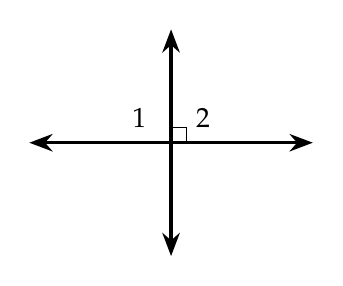
\begin{tikzpicture}[scale=0.9]\draw[very thick,{Stealth}-{Stealth}] (-2,0)--(2,0);\draw[very thick,{Stealth}-{Stealth}] (0,-1.6)--(0,1.6);\node at (-0.45,0.35){$1$};\node at (0.45,0.35){$2$};\draw (0,0)--(0.22,0)--(0.22,0.22)--(0,0.22);\end{tikzpicture}\end{column}\begin{column}{0.54\textwidth}\onslide<1->{\key{Perpendicular} lines meet at a \key{right angle}: \ $a \perp b$}\par\medskip
\onslide<2->{The little \key{square} in a picture marks a right angle.}\par\medskip\end{column}\end{columns}
\end{frame}
\begin{frame}{Linear pair of congruent angles}
\begin{columns}[c]\begin{column}{0.44\textwidth}\centering 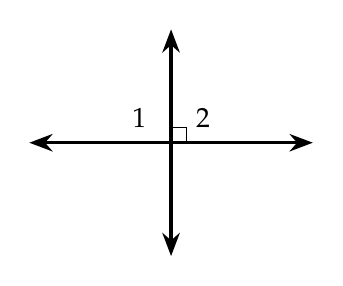
\begin{tikzpicture}[scale=0.9]\draw[very thick,{Stealth}-{Stealth}] (-2,0)--(2,0);\draw[very thick,{Stealth}-{Stealth}] (0,-1.6)--(0,1.6);\node at (-0.45,0.35){$1$};\node at (0.45,0.35){$2$};\draw (0,0)--(0.22,0)--(0.22,0.22)--(0,0.22);\end{tikzpicture}\end{column}\begin{column}{0.54\textwidth}\onslide<1->{$\angle 1$ and $\angle 2$ form a linear pair: \ $m\angle 1 + m\angle 2 = 180^\circ$}\par\medskip
\onslide<2->{If $\angle 1 \cong \angle 2$: each is $180 \div 2 = \ans{90^\circ}$}\par\medskip
\onslide<3->{\defn{Two lines that form a linear pair of congruent angles are \key{perpendicular}.}}\par\medskip\end{column}\end{columns}
\end{frame}
\begin{frame}{Two lines perpendicular to the same line}
\onslide<1->{In a plane: $a \perp t$ and $b \perp t$ $\Rightarrow$ \key{$a \parallel b$}}\par\medskip
\onslide<2->{Why: corresponding angles are both $90^\circ$, so they are congruent.}\par\medskip
\end{frame}
\begin{frame}{Distance from a point to a line}
\begin{columns}[c]\begin{column}{0.44\textwidth}\centering 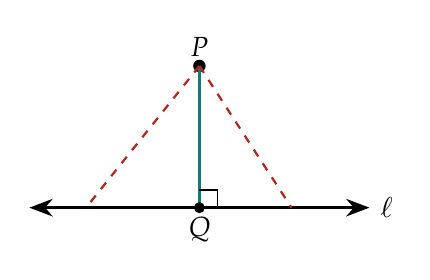
\begin{tikzpicture}[scale=0.9]\draw[very thick,{Stealth}-{Stealth}] (-2.4,0)--(2.4,0) node[right]{$\ell$};\fill (0,2) circle(2.5pt) node[above]{$P$};\draw[very thick,fteal] (0,2)--(0,0);\fill (0,0) circle(2.2pt) node[below]{$Q$};\draw (0,0)--(0.25,0)--(0.25,0.25)--(0,0.25);\draw[thick,dashed,fred] (0,2)--(-1.6,0) (0,2)--(1.3,0);\end{tikzpicture}\end{column}\begin{column}{0.54\textwidth}\onslide<1->{Drop a segment from $P$ straight down to $\ell$: $\overline{PQ} \perp \ell$}\par\medskip
\onslide<2->{Every slanted path is \textbf{longer} than $PQ$.}\par\medskip
\onslide<3->{\defn{Distance from a point to a line $=$ length of the \key{perpendicular} segment.}}\par\medskip\end{column}\end{columns}
\end{frame}
\begin{frame}{Watch out}
\onslide<1->{\warn{Only the \textbf{perpendicular} segment measures the distance to a line --- not a slanted one.}}\par\medskip
\end{frame}
\begin{frame}{}
\begin{yourturn}Point $P(3, 5)$ and the line $y = 1$. \ What is the distance from $P$ to the line?\end{yourturn}\par\medskip
\onslide<2->{Go straight down to $(3, 1)$: \ distance $= 5 - 1 = \ans{4}$}\par\medskip
\end{frame}
\closeframe{\begin{itemize}\setlength\itemsep{8pt}
\item \key{Perpendicular} lines meet at $90^\circ$.
\item Linear pair of congruent angles $\Rightarrow$ perpendicular.
\item Distance to a line $=$ the \key{perpendicular} segment, the shortest path.
\end{itemize}}
\end{document}
